\documentclass{article}

% \usepackage{natbib}

\usepackage[utf8]{inputenc}
\usepackage[
backend=biber,
style=alphabetic,
sorting=ynt
]{biblatex}
\usepackage{comment}
\usepackage{csquotes}


%%proof at end


\usepackage[ruled,vlined]{algorithm2e}
\addbibresource{citations.bib}
\usepackage[english]{babel}
\usepackage{url}
\usepackage{mathtools}
\usepackage{enumitem}
\usepackage{dsfont}
\usepackage{bbm}
\usepackage{float}
\usepackage{stmaryrd}
\usepackage[utf8]{inputenc}
\usepackage[T1]{fontenc}
\usepackage{placeins}
\usepackage{amsmath, amsfonts, amssymb}
\usepackage{graphicx}
\usepackage{caption}
\usepackage[nottoc]{tocbibind}
\usepackage[ruled,vlined]{algorithm2e}
\newcommand\tab[1][0.5cm]{\hspace*{#1}}
\newcommand\reals{\mathbb{R}}
\usepackage{amsthm}
\newcommand\tp{\Tilde{P}}
\newcommand\JP{P^{\alpha,\beta}}

\newcommand\tmu{\Tilde{\mu}}
\DeclareMathOperator{\supp}{supp}

\newtheorem{theorem}{Theorem}
\newtheorem{define}{Definition}
\newcommand\jp{p_t^{\alpha,\beta}}
\newtheorem{lemma}[theorem]{Lemma}
%\newtheorem{assumption}[theorem]{Assumption}
\newtheorem{corolary}[theorem]{Corollary}
%\newtheorem{example}[theorem]{Example}

\newtheorem{remark}[theorem]{Remark}
\usepackage[utf8]{inputenc} % allow utf-8 input
\usepackage[T1]{fontenc}    % use 8-bit T1 fonts
%\usepackage{hyperref}       % hyperlinks
\usepackage{url}            % simple URL typesetting
\usepackage{booktabs}       % professional-quality tables
\usepackage{amsfonts}       % blackboard math symbols
\usepackage{nicefrac}       % compact symbols for 1/2, etc.
\usepackage{microtype}      % microtypography

\usepackage{appendix}


\usepackage{empheq}
\usepackage{xcolor, color, colortbl}
\usepackage{framed}
\usepackage{pifont}
\newcommand{\cmark}{\ding{51}}%
\newcommand{\xmark}{\ding{55}}%
\usepackage{enumitem}
% For figures
\usepackage{graphicx} % more modern
%\usepackage{epsfig} % less modern

% to avoid too much space after the algorithm
% \setlength{\textfloatsep}{10pt}% Remove \textfloatsep

\usepackage{nicefrac}
\usepackage{booktabs}
\usepackage{multirow}
\usepackage{rotating}
\usepackage{nccmath}

\usepackage[tikz]{bclogo}
\usepackage{wasysym}

%\SetAlFnt{\normalsize}

\definecolor{mydarkblue}{rgb}{0,0.08,0.45}
\usepackage[
    colorlinks=true,
    linkcolor=mydarkblue,
    citecolor=mydarkblue,
    filecolor=mydarkblue,
    urlcolor=mydarkblue,
    pdfview=FitH]{hyperref}
% smaller url fonts
\usepackage{url}
\usepackage{relsize}
\usepackage{ICLR/iclr2022_conference}
\renewcommand*{\UrlFont}{\ttfamily\smaller\relax}

\newcommand{\blue}{\color{blue}}
\def\xx{{\boldsymbol x}}
\def\yy{{\boldsymbol y}}
\def\zz{{\boldsymbol z}}
\def\qq{{\boldsymbol q}}
\def\dd{{\boldsymbol d}}
\def\XX{{\boldsymbol X}}
\def\YY{{\boldsymbol Y}}
\def\ZZ{{\boldsymbol Z}}
\def\aa{{\boldsymbol a}}
\def\bb{{\boldsymbol b}}
\def\rr{{\boldsymbol r}}
\def\cc{{\boldsymbol c}}
\def\qq{{\boldsymbol q}}
\def\WW{{\boldsymbol W}}
\def\KK{{\boldsymbol K}}
\def\II{{\boldsymbol I}}
\def\yy{{\boldsymbol y}}
\def\vv{{\boldsymbol v}}
\def\uu{{\boldsymbol u}}
\def\ww{{\boldsymbol w}}
\def\zz{{\boldsymbol z}}
\def\SS{{\boldsymbol S}}
\def\BB{{\boldsymbol B}}
\def\AA{{\boldsymbol A}}
\def\CC{{\boldsymbol C}}
\def\MM{{\boldsymbol M}}
\def\DD{{\boldsymbol D}}
\def\PP{{\boldsymbol P}}
\def\TT{{\boldsymbol T}}
\def\VV{{\boldsymbol V}}
\def\bphi{{\boldsymbol \phi}}
\def\QQ{{\boldsymbol Q}}
\def\UU{{\boldsymbol U}}
\def\HH{{\boldsymbol H}}
\def\balpha{{\boldsymbol \alpha}}
\def\bpsi{{\boldsymbol \psi}}
\def\LLambda{{\boldsymbol \Lambda}}
\def\eeps{{\boldsymbol \varepsilon}}
\def\dif{\mathop{}\!\mathrm{d}}
\def\Proba{\mathbb{P}}
\def\MP{\mu_{\mathrm{MP}}}

\def\RR{{\mathbb R}}
\def\EE{{\mathbb{E}}}
\newcommand{\Econd}{\mathbf{E}}
\renewcommand{\gg}{\boldsymbol{g}}
\renewcommand{\vec}{\mathbf{vec}}
\DeclareMathOperator{\prox}{\mathbf{prox}}
\DeclareMathOperator{\tr}{tr}
\def\defas{\stackrel{\text{def}}{=}}
\DeclareMathOperator*{\dom}{dom}
% \DeclareMathOperator*{\supp}{supp}
\DeclareMathOperator*{\Fix}{Fix}
\DeclareMathOperator*{\Var}{Var}
\DeclareMathOperator*{\Span}{\mathbf{span}}
\DeclareMathOperator*{\Deg}{{deg}}
\DeclareMathOperator*{\Trace}{{tr}}

% \newcommand{\xdownarrow}[1]{%
%   {\left\downarrow\vbox to #1{}\right.\kern-\nulldelimiterspace}
% }


\newcommand*\mybluebox[1]{\colorbox{myblue}{\hspace{1em}#1\hspace{1em}}}

\DeclareMathOperator*{\argmin}{{arg\,min}}
\DeclareMathOperator*{\minimize}{minimize}
\DeclareMathOperator*{\diag}{\mathbf{diag}}

\definecolor{myblue}{HTML}{D2E4FC}
\definecolor{Gray}{gray}{0.92}
    
\newtheorem{definition}{Definition}
\newtheorem{example}{Example}
% \newtheorem{remark}{Remark}
\newtheorem{assumption}{Assumption}
% \newtheorem{lemma}{Lemma}
% \newtheorem{proof}{Proof}
\newtheorem{proposition}{Proposition}
% \newtheorem{theorem}{Theorem}


\usepackage{thmtools}
\usepackage{thm-restate}

\usepackage{wrapfig}

\declaretheorem[name=Theorem,numberwithin=section]{thm}
\declaretheorem[name=Proposition,numberwithin=section]{prop}

\DeclareDocumentCommand{\Prto} {o} {
  \IfNoValueTF {#1}
  {\overset{\Pr}{\longrightarrow}}
  { \xrightarrow[ #1 \to \infty]{\Pr }}
}


\title{Robust Average Case Analysis on the Non-Strongly Convex Setting \\
or the wonders of the Nesterov method}


\author{Leonardo Cunha
\and Gauthier Gidel \\
\and Fabien Pedregosa \\
\and Courtney Paquette \\
\and Damien Scieur}
\date{May 2021}

\begin{document}
\maketitle
\begin{abstract}
    Recent works \cite{pedregosa2020acceleration,paquette2020halting,scieur2020universal} have studied the convergence properties of first order optimization methods on distributions of quadratic problems. \\
    In this work we contrast the Nesterov Accelerated Method \cite{nesterov2003introductory} and a family of methods we derive,  namely the Generalized Chebyshev method, which are optimal when the problem's expected spectral distribution is a beta weight.\\
    As the exact spectral distribution is too strong of an hypothesis to enable practical decision making regarding the choice of algorithm, we compare the methods under a weaker hypothesis on the distribution and notice that in the average case a problem's complexity is driven to the concentration of the problem's eigenspectra around the edges of it's support, in contrast to  only the values of the edges in the worst case. \\
    We show that the Nesterov is \textbf{robustly} close to optimum convergence, in the asymptotic sense
\end{abstract}
\section{Introduction}
The analysis of the average complexity of algorithms is an old feature of computer science. Notably, the quicksort algorithm presents worst-case complexity of $O(n^2)$, but average case complexity of $O(n\log n)$ and is  empirically faster than HeapSort or MergeSort. Average case complexity also drives much of the decisions made in cryptography \cite{bogdanov2006average}\\
The average case analysis of optimization algorithm has stayed an unexplored problem for long because of the ill-defined notion of a distribution over the optimization problems. Recently though, \cite{pedregosa2020acceleration} has derived a framework to systemically evaluate the complexity of first order methods on distributions of quadratic minimization problems by tying the average of the residuals to the \textit{expected spectral distribution} of the problem, which is a well studied object on Random Matrix Theory. \\
\cite{paquette2020halting} has expanded on this work by introducing a new generative model for the problems and deriving the average complexity of the Nesterov Accelerated Method on a particular distribution and showing the strong concentration of the metrics around their expected value. \\
\cite{scieur2020universal} has shown that for a strongly convex problem with eigenvalues supported on a contiguous interval, the optimal average case complexity is asymptotically equal to the one given by the Polyak Heavy Ball method in the worst-case.  

%%There are more works on the average case I did not introduce , such as those done on the stochastic setting and on CG. They are not directly relevant to our work, IDK if I should introduce them aswell 

\paragraph{}
In the non-strongly convex case, optimization drastically slows down, as gradient descent presents worst case convergence in $\Theta(\frac{1}{n})$ and Nesterov is $\Theta(\frac{1}{n^2})$, which matches a lower bound on worst case convergence up to a constant factor. \\
We believe the non strongly convex, worst case scenario is very pessimistic, especially in high dimensions where the problem has enough degrees of freedom to be highly adversarial [citation of the tutorial here+ quotation marks]. Further, as we are dealing with the sublinear convergence of large scale algorithms,  accelerated sublinear rates may be the difference between problems that are computationally feasible and those who are not  \\
A drawback on average case analysis is that it relies, \textit{à priori}, on a much stronger hypothesis, the shape of the \textit{expected spectral distribution} as we'll see, when compared to the worst case analysis, that relies only on the values of the edges of this distribution. \\
We show that the main aspects of the convergence, which from an optimization point view are the asymptotic rates, are determined by a low dimensional characterization of the distribution. Parametrizing the distributions in terms of the \textbf{concentration} of the eigenvalues around the edges, allow us to effectively determine the precise rates for all continuous distributions supported in an interval $]0,L[$, \\
We can then compare algorithms robustly, allowing an effective choice of algorithms under a more realistic lack of information on the eigenspectra. \\
%Considering that, we were motivated to look for average case speed ups or  similar universality results on the non-strongly convex setting, which is  also a more relevant model for the optimization problems commonly found on machine learning. A positive answer would diminish the relevance of the average case analysis, as the average rates would be very similar to the worst case ones.\\
%As we found out, in this setting different distributions gave origin to different sublinear rates, indeed the worst case complexity can be arbitrarily pessimistic depending on the distribution as we'll see. Our concern for universality got changed into a concern for robustness. We can thus phrase the question this paper tries to answer as the search for the method who has "good" performance under the broadest set of hypothesis over the problem distribution. \\
\paragraph{}
In the following, we will first present the average case framework first introduced by \cite{pedregosa2020acceleration}, we'll then present some basic universality results showing that the complexity is driven by the concentration the eigenvalues near the edges of the support. \\
We will then compute the optimal rates and those of the Nesterov in terms of the concentration parameters, and we observe we can find the worst case rates as limit on the average case. \\
Finally we'll state our main results : the Nesterov accelerated method asymptotic rate is close to the optimal one for relatively high concentrations of the eigenspectra near $0$, only a $\log$ term under a standard hypothesis. This means the Nesterov method is a very robust choice on practical scenarios.


\begin{figure}[H]
    \centering
    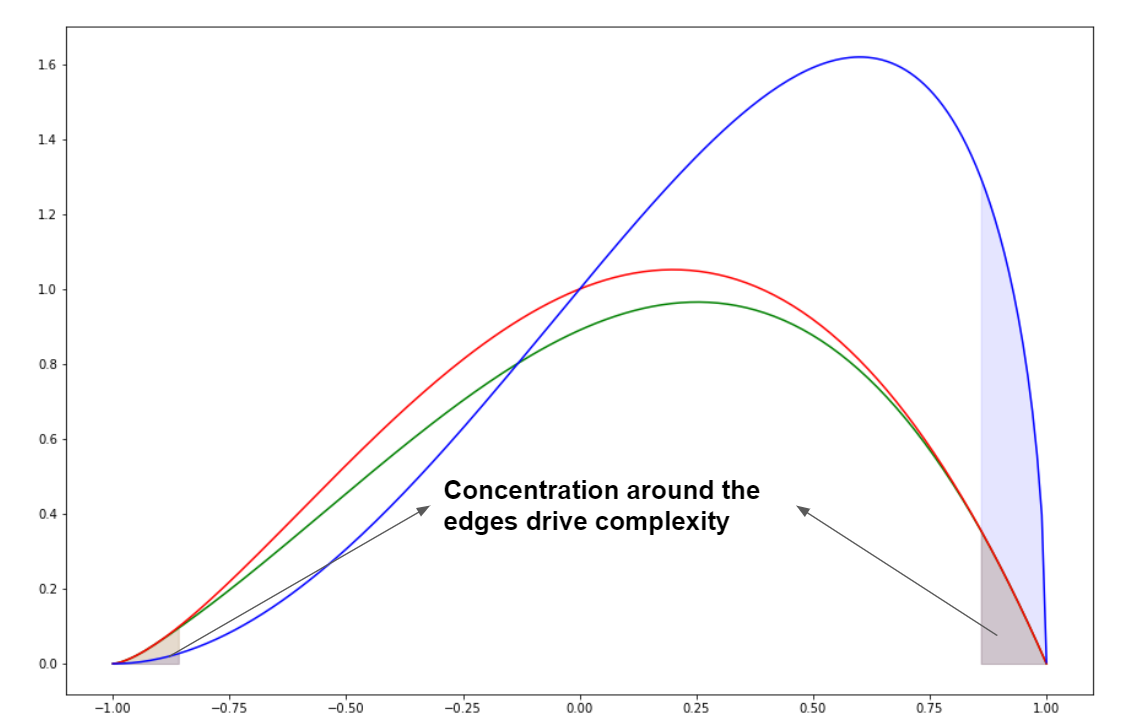
\includegraphics[width=8 cm]{imgs/concentration.PNG}
    \caption{The average case rates for non-strongly problems is determined by the eigenvalue concentration around the edges of the support }
    \label{fig:my_label}
\end{figure}

\section{Average-Case Analysis} \label{sec:methods}


In this section we introduce the average-case analysis framework for random quadratic problems.
The main result is Theorem~\ref{thm: metrics}, which relates the expected error with other quantities that will be easier to manipulate, such as the residual polynomial. This is a convenient representation of an optimization method that will allow us in the next section to pose the problem of finding an optimal method as a best approximation problem in the space of polynomials.


Let $\HH \in \RR^{d \times d}$ be a random symmetric positive-definite matrix and $\xx^\star \in \RR^d$ a random vector. These elements determine the following (random) quadratic minimization problem
\begin{empheq}[box=\mybluebox]{equation*}\tag{OPT}\label{eq:quad_optim}
  \vphantom{\sum_0^i}\min_{\xx \in \RR^d} \Big\{ f(\xx) \defas\!\mfrac{1}{2}(\xx\!-\!\xx^\star)^\top\!\HH(\xx\!-\!\xx^\star) \Big\}\,.
\end{empheq}
Our goal is to quantify the expected error $\EE \|\xx_t - \xx^\star\|$, where $\xx_t$ is the $t$-th update of a first-order method starting from $\xx_0$ and $\EE$ is the expectation over the random $\HH, \xx_0, \xx^\star$.



\begin{remark} The expectation in the expected error ${\EE \|\xx_t - \xx^\star\|^2}$ is over the inputs and not over any randomness of the algorithm, as would be common in the stochastic literature. In this paper we will only consider deterministic algorithms.
\end{remark}


To solve \ref{eq:quad_optim}, we will consider \emph{first-order methods}. These are methods in which the sequence of iterates $\xx_t$ is in the span of previous gradients, i.e.,
\begin{equation} \label{eq:first_order_methods}
    \xx_{t+1} \in \xx_0 + \Span\{ \nabla f(\xx_0), \ldots, \nabla f(\xx_t)  \}\, .
\end{equation}
This class of algorithms includes for instance gradient descent and momentum, but not quasi-Newton methods, since the preconditioner could allow the iterates to go outside of the span. Furthermore, we will only consider \emph{oblivious} methods, that is, methods in which the coefficients of the update are known in advance and don't depend on previous updates. This leaves out some methods that are specific to quadratic problems like conjugate gradient.


\paragraph{From First-Order Method to Polynomials.}
There is an intimate link between first order methods and polynomials that simplifies the analysis on quadratic objectives. Using this link, we will be able to assign to each optimization method a polynomial that determines its convergence. The next Proposition gives a precise statement:
% The following proposition states this relationship which relates the error at iteration $t$ with the error at initialization and the residual polynomial.


\begin{restatable}{prop}{linkalgopolynomial}
    \label{prop:link_algo_polynomial} \parencite{hestenes1952methods}
    Let $\xx_t$ be generated by a first-order method. Then there exists a polynomial $P_t$ of degree $t$ such that $P_t(0) = 1$ that verifies
    \begin{equation}\label{eq:polynomial_iterates}
        \vphantom{\sum^n}\xx_{t}-\xx^\star = P_t(\HH)(\xx_0-\xx^\star)~.
    \end{equation}
\end{restatable}

\begin{remark} \label{rmk: momentum based}
If the first-order method is further a \textbf{momentum method}, i.e.:
$$
    \xx_{t+1}=\xx_t+m_t(\xx_t-\xx_{t-1})+h_t\nabla f(\xx_t)
$$.
We can determine the polynomials by the recurrence $P_0=1$ and:
    \begin{equation*}
        P_{t+1}(\lambda)=(1+m_t)P_t(\lambda)+h_t\lambda P_t(\lambda)-m_tP_{t-1}(\lambda)
    \end{equation*}
We note that while most popular F.O.M's can be posed a momentum method, Nesterov cannot.
\end{remark}

Following \textcite{fischer1996polynomial}, we will refer to this polynomial $P_t$ as the \emph{residual polynomial}.




A convenient way to collect statistics on the spectrum of a matrix is through its \emph{empirical spectral distribution}, which we now define. 


\begin{definition}
(\textbf{Weighted/Expected spectral distribution}). 
Let $\HH$ be a random matrix with eigenvalues $\{\lambda_1, \ldots, \lambda_d\}$. The \textbf{empirical spectral distribution} of $\HH$, called ${\mu}_{\HH,\;\alpha}$, is the probability measure
\begin{equation}\label{eq:wighted_spectral_density}
    \mu_{\HH} \defas \frac{1}{d}{\textstyle{\sum_{i=1}^d}} \delta_{\lambda_i},
\end{equation}
where $\delta_{\lambda_i}$ is the Dirac delta, a distribution equal to zero everywhere except at $\lambda_i$ and whose integral over the entire real line is equal to one.

Since $\HH$ is random, the empirical spectral distribution $\mu_\HH$ is a random measure (a random variable in the space of measures). Its expectation over $\HH$ is called the \textbf{expected spectral distribution} (e.s.d.) and we denote it
\begin{equation}
\mu \defas \EE_{\HH}[\mu_{\HH}]\,.
\end{equation}
\end{definition}

We can link the e.s.d. of $\HH$ to the convergence of a first order method on the distribution of $\HH$ In the following we'll consider $x_0-x^\star$ and $\HH$ to be independent, with $x_0-x^\star$ sampled isotropically. This isotropic hypothesis is not necessary and we could derive a similar analysis for  more general distribution  of $x_0-x^\star$.

\begin{restatable}{thm}{metrics} \label{thm: metrics}
Let $\xx_t$ be generated by a first-order method associated to the polynomial $P_t$,  $\mu$ the  e.s.d. of $H$ and $\mathbb{E}[(\xx_0-\xx^\star)(\xx_0-\xx^\star)^T]=R^2\textbf{I}$ Then we can write the convergence metrics at time step  $t$ as:
\begin{align}\label{eq:error_norm_x}
  \mathbb{E}[\|\xx_t-\xx^\star\|^2] &= { R^2} \int {P_t^2(\lambda) d\mu(\lambda)} \\
    \mathbb{E}[f(\xx_t)-f(\xx^\star)]&=R^2\int P_t^2(\lambda)\lambda d\mu(\lambda)\\
    \mathbb{E}[||\nabla f(\xx_t)||^2_2]&=R^2\int P_t^2(\lambda)\lambda^2d\mu(\lambda) 
\end{align}
\end{restatable}
This shows that the polynomials are an excellent abstraction: in the following we'll refer directly to the polynomials associated to a given method and omit the $R^2$ term associated to the initialization. We'll simply refer to metric $l$ as the metric associated to the added $\lambda^l$ term, i.e. the gradient norm is metric $l=2$\\
\paragraph{}
This framework is further linked to the field of \textbf{orthogonal polynomials} by the following proposition which gives a construction of an optimal method w.r.t. a given distribution 
\begin{restatable}{prop}{optimality}\cite{pedregosa2020acceleration}
 \label{prop: optimality}
 Let $P_t^\star$ be defined as
 \begin{equation}
     P_t^\star:={\arg \min}_{P_t(0)=1} \int P_t^2(\lambda) \lambda^l d\nu(\lambda)
 \end{equation}
 then $(P_t^\star)$ is the family of residual orthogonal polynomials w.r.t. to $\lambda^{a+1}d\nu$
\end{restatable}

This theorem further implies that the  optimal first-order method is a momentum method as Favard's theorem \cite{marcellan2001favard} tells us the residual orthogonal polynomials w.r.t. a given distribution can be related through a \textbf{three term recurrence}:

\begin{equation}
    P_{t+1}(\lambda)=a_tP_t(\lambda)+b_t\lambda P_t(\lambda)+(1-a_t)P_{t-1}(\lambda)
\end{equation}
Following remark \ref{rmk: momentum based}, the optimal method is derived from this recurrence as:
\begin{equation}
    \xx_{t+1}=\xx_t+(a_t-1)(\xx_t-\xx_{t-1})+b_t\nabla f(\xx_t)
\end{equation}



\section{Generalized Chebyshev method}
Being able to write the rates in terms of the \textit{expected spectral distribution} ties the average case framework to the field of \textit{random matrix theory}. Indeed, because of results from this field, certain e.s.d's are considered more natural than others. We illustrate this and motivate following considerations with:
\begin{prop}[Marchenko Pastur Theorem]
Let $X_n$ be a $m\times n$ random matrix with $X_{ij}$ i.i.d with variance $\sigma^2$ and $Y_n=\frac{1}{n}X_nX_n^T$. Let $\mu_n$ be the expected spectrum of $Y_n$, then, as $n\rightarrow\infty$$\frac{m}{n} \rightarrow r$:

\begin{align*}
&\mu_n\xrightarrow{\text{weakly}}{}\max(0,1-\frac{1}{r})\delta_0+\mu_{MP} \\
&d\mu_{MP}(\lambda)=\frac{1}{2\pi\sigma^2}\frac{\sqrt{(\lambda^+-\lambda)(\lambda-\lambda^-)}}{r\lambda}
\end{align*}
With $\lambda^+=\sigma^2(1+\sqrt{r})^2$, $\lambda^-=\max(0,\sigma^2(1-\sqrt{r})^2)$

\end{prop}
The Marchenko Pastur distribution $\mu_{MP}$ can be considered a natural first model for e.s.d's as it arises universally, note there's no specific distribution of $X_{ij}$ considered, from i.i.d. noise in the matrix entries.\\
When $r=1 d\mu_{MP}\propto \lambda^{-1/2}\sqrt{\lambda^+-\lambda}$, Though practical e.s.d's diverge from it, the concentration near $0$ is often verified.
\cite{pedregosa2020acceleration} first derived the optimal method wrt. $\mu_{MP}$, and \cite{paquette2020halting} derived Nesterov's rates under it. As we are mainly concerned with being robust, a natural step is to consider the Beta weights $d\mu(\lambda)\propto\lambda^\xi(L-\lambda)^\tau$ but we are mainly interested in distributions with similar concentrations near $0$, i.e. $\xi\approx -1/2$.\\
The optimal method w.r.t. $\mu$ and metric $l$ is associated to a shifted Jacobi polynomial $\tp_t^{\alpha,\beta}$ with $\beta=\xi+l+1, \alpha=\tau$. When $\alpha=\beta=-1/2$ we retrieve the \textit{Chebyshev Method} \cite{hestenes1952methods}, so we call this the Generalized Chebyshev Method
We derive the coefficients associated to this method in appendix \ref{jacobi recurrence}.\\
\begin{remark}
The Generalized Chebyshev also takes the largest eigenvalue $L$ as a parameter, but the rates we'll show are robust to an \textit{overestimation} of $L$
\end{remark}

\section{Robust Average Case Rate}
We will establish our assumption over the spectral distributions. It effectively allows us to parametrize all of our distributions of interest in a way that characterize the asymptotic convergence, diving them into equivalence classes .

\begin{assumption}
We will write $\nu_{\tau,\xi}$ for a continuous distribution supported in $(0,L]$ s.t. $\nu_{\tau,\xi}'(x)>0$ for $x\in [0,L]$, $d\nu_{\tau,\xi}=\Theta( \lambda^\xi)$ near $0$ and $d\nu_{\tau,\xi}=\Theta( (L-\lambda)^\tau)$ near $L$. 
\label{assumption}
\end{assumption}

We single out from each of these classes the beta distributions for which we can compute the rates, then show the rates to be the same inside $\nu_{\tau,\xi}$.\\ 

\paragraph{}
We show that $\nu_{\tau,\xi}$ indeed behaves like an equivalence class when considering the asymptotics of the convergence of a Jacobi method: only the concentrations near the edge matter:

\begin{restatable}{theorem}{robustjacobi}[Robustness of Jacobi]\label{thm: jacobirates}
A Generalized Chebyshev Method with parameters $(\alpha,\beta)$ applied to a problem with e.s.d. as in assumption \ref{assumption} has rates:

\begin{align}
\mathbb{E}[f(\xx_t)-f(\xx^\star)]&\sim L\cdot C^{\alpha,\beta}_{1,\nu}
    \left\{\begin{array}{ll}
    t^{-1-2\beta} &\mbox{if } 
		  \alpha<\tau+1/2 \text{ and } \beta <\xi+3/2\\
		  t^{-2(\xi+2)}\log t& \mbox{if } 
		  \alpha=\tau+1/2 \text{ and } \beta =\xi+3/2\\
		  t^{2(\max\{\alpha-\beta-\tau,-\xi-1\}-1)}& \mbox{if } 
		  \alpha>\tau+1/2 \text{ or } \beta >\xi+3/2
	\end{array}\right.\\
	\mathbb{E}[||\nabla f(\xx_t)||^2_2]&\sim L^2\cdot C^{\alpha,\beta}_{2,\nu}
        \left\{\begin{array}{ll}
    t^{-1-2\beta} &\mbox{if } 
		  \alpha<\tau+1/2 \text{ and } \beta <\xi+5/2\\
		  t^{-2(\xi+3)}\log t& \mbox{if } 
		  \alpha=\tau+1/2 \text{ and } \beta =\xi+5/2\\
		  t^{2(\max\{\alpha-\beta-\tau,-\xi-2\}-1)}& \mbox{if } 
		  \alpha>\tau+1/2 \text{ or } \beta >\xi+5/2
	\end{array}\right.
\end{align}
Where $C^{\alpha,\beta}_\nu$ is a distribution dependent constant.
\end{restatable}
\begin{figure}[H]
    \centering
    %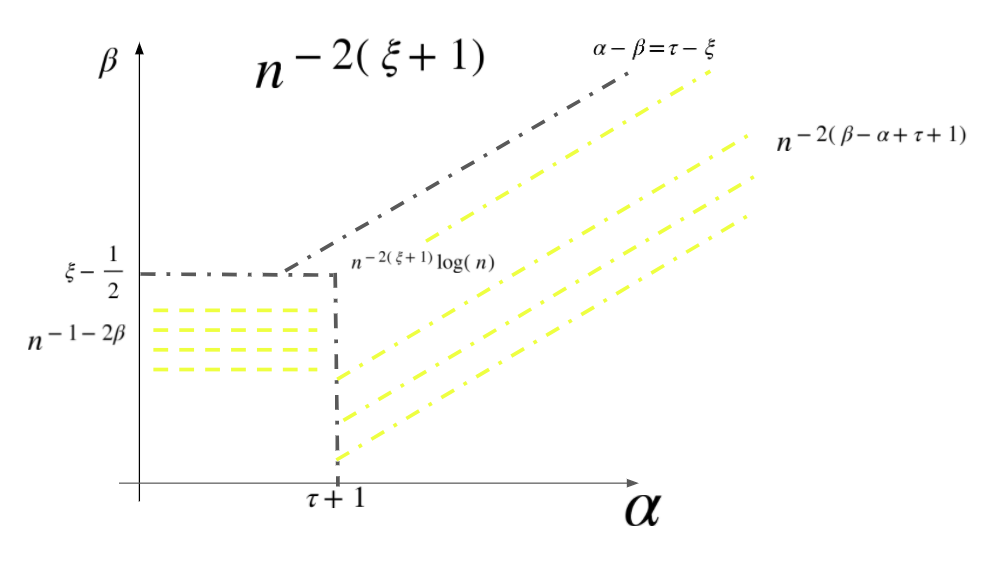
\includegraphics[width=10 cm]{imgs/diagram.PNG}
    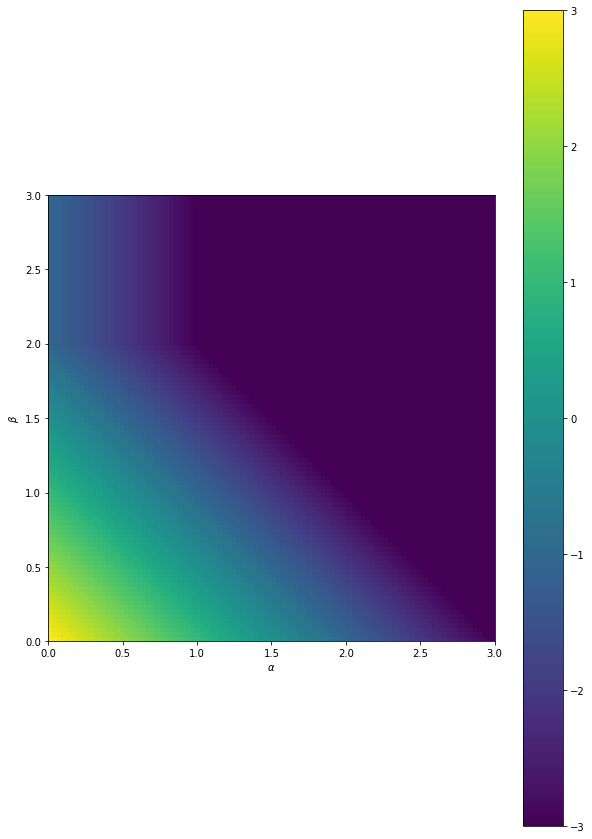
\includegraphics[width=4 cm]{imgs/colormap.png}
    
    \caption{Colormap for the function value rates  for the Marchenko Pastur distribution. The color represents the negative exponent, e.g. lower is better.}
    \label{fig:my_label2}
\end{figure}



Theorem \ref{thm: optimality} shows that a proper choice of $\alpha,\beta$ can indeed make the Jacobi polynomial asymptotically optimal w.r.t. to any $\nu_{\tau,\xi}$. 

\begin{restatable}{theorem}{jacoptimal}[Optimality of Jacobi]\label{thm: optimality}
Let $\nu$ follow assumption \ref{assumption}. \\
The optimal asymptotic rate for $\mathbb{E}[f(\xx_t)-f(\xx^\star)]$ is $t^{-2(\xi+2}$ and is attained by the Chebyshev Method with parameters $(\tau,\xi+2)$. \\
The optimal rate for $\mathbb{E}[||\nabla f(\xx_t)||^2_2]$ is $t^{-2(\xi+3}$ and is attained by the Chebyshev Method with parameters $(\tau,\xi+3)$.
\end{restatable}

For the function value ($l=1$), we find rates that approach $t^{-2}$ as $\xi\rightarrow -1$, showing the worst case as a limit (over the considered distribution) on the average case.
\begin{remark}
We can contextualize our results on the field of orthogonal polynomials as asymptotics on the values of the \textit{Christoffel Functions} at $0$ \cite{totik2005orthogonal}:

\begin{equation}
    \lambda_t(\mu,x)=\inf_{P_t(x):=1,\deg(P_t)\leq t}\int P_t^2 d\mu=\Big( \sum_{k=0}^tp_k(x;\mu)^2\Big)^{-1}
\end{equation}
 For the equivalence classes $\nu_{\tau,\xi}$
\end{remark}
We remark that the above theorems imply that, at least asymptotically, the Jacobi method is robust for a suboptimal choice of parameters up to $1/2$ below the optimal choice of $\beta$ and infinitely above. \\
For completeness, we also derive worst case rates for the Jacobi method:

\begin{restatable}{prop}{worstcase}[Worst case Jacobi rates]
Let $H$ be a convex, L-smooth function. Then, For the Generalized Chebyshev Method with parameters $(\alpha,\beta)$ we have $f(\xx_t)-f(\xx^\star)=O(Lt^{v_1(\alpha,\beta)})$, and $||\nabla f(\xx_t)-f(\xx^\star)||^2=O(L^2t^{v_2(\alpha,\beta)})$, with:

\begin{align}
    v_1(\alpha,\beta)&=\left\{
    \begin{array}{cc}
           2(\alpha-\beta) &\text{if} \hspace{0.5 cm} \alpha>\beta-1 \\
         -1-2\beta, \hspace{1 cm} &\text{if} \hspace{0.5 cm} \alpha\leq \beta-1\hspace{0.5 cm} \beta\leq \frac{1}{2}\\
         -2, \hspace{1 cm} &\text{if} \hspace{0.5 cm} \alpha\leq\beta-1\hspace{0.5 cm} \beta\geq \frac{1}{2} 
    \end{array}
    \right\\
    v_2(\alpha,\beta)&=\left\{
    \begin{array}{cc}
           2(\alpha-\beta) &\text{if} \hspace{0.5 cm} \alpha>\beta-2 \\
         -1-2\beta, \hspace{1 cm} &\text{if} \hspace{0.5 cm} \alpha\leq \beta-2\hspace{0.5 cm} \beta\leq 3/2\\
         -4, \hspace{1 cm} &\text{if} \hspace{0.5 cm} \alpha\leq\beta-2\hspace{0.5 cm} \beta\geq 3/2
    \end{array}
    \right . 
\end{align}
\end{restatable}


For the function value ($l=1$) and a reasonable choice of $\alpha,\beta$ this means effectively that the worst case rates are $t^{-2}$ 

\paragraph{}
\cite{nesterov2003introductory} has shown that the Nesterov matches up to a a constant factor a lower bound on the worst case complexity of non strongly convex problems. A natural question is if this performance would translate to good average case rates. \\
We'll extend \cite{paquette2020halting} proof for the Nesterov method under the MP distribution  
\begin{restatable}{thm}{nesterovrates}
Let $\nu$ as in assumption \ref{assumption}, then, for the Nesterov method:
\begin{align}
    \mathbb{E}[f(\xx_t)-f(\xx^\star)]&\sim C'_{1,\nu}
    \Big\{\begin{array}{ll}
		  t^{-2(\xi+2)}& \mbox{if } 
		  \xi<-1/2\\
		  t^{-3}\log t& \mbox{if } 
		  \xi=-1/2\\
		  t^{-(\xi+7/2)}& \mbox{if } 
		  \xi>-1/2
	\end{array}\\
	\mathbb{E}[||\nabla f(\xx_t)||^2_2] &\sim C'_{2,\nu}
		  t^{-(\xi+9/2)}
\end{align}
\end{restatable}
The optimality gap of nesterov is $t{\xi+l-1/2}$, when $\xi+l>1/2$, $\log t$ when $\xi+l=1/2$ and $0$ otherwise.
This shows that Nesterov is almost optimal when the concentrations near $0$ are relatively high, i.e. low $\xi$\\
Observe we again find the $t^{-2}$ rates for the function value when $\xi\rightarrow-1$

\begin{table}[H]
    \centering
    \begin{tabular}{c|c|c|c}
         $(\tau,\xi)$/Method& Chebyshev ($\frac{1}{2},\frac{5}{2}$) & Chebyshev ($\frac{1}{2},\frac{3}{2}$) &  Nesterov  \\
         \hline
         ($\frac{3}{2},\frac{1}{2}$)&$t^{-5}$ & $t^{-4}$ & $t^{-4}$\\
         \hline
         ($\frac{1}{2},\frac{1}{2}$)&$t^{-3}$ & $t^{-3}$ & $t^{-3}\log t$
         
    \end{tabular}
    \caption{Caption}
    \label{tab:theoretic rates}
\end{table}


\section{Experiments}
We estimated empirically the asymptotic rates from table \ref{tab:theoretic rates} by doing linear regression on the log-log domain. \\
We synthesize the e.s.d's  either by means of the Marchenko Pastur that enables us to simulate $(\tau,\xi)$ values of $(1/2,3/2)$ and $(1/2,5/2)$. Other values are simulated by sampling from the corresponding Beta distribution and applying a random rotation to the diagonal matrix comprising those samples.\\ 
As ours are the asymptotic rates on the infinite dimensional case, i.e. we take $d\rightarrow \infty$ and then $t \rightarrow \infty$, they are representative of the experiments on the regime $t<d$.

\begin{figure}[H]
    \centering
    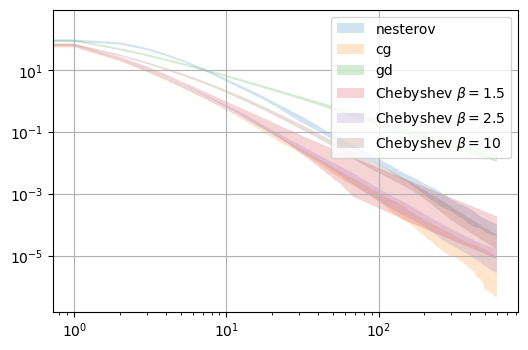
\includegraphics[width=5 cm]{imgs/mp/log f.png}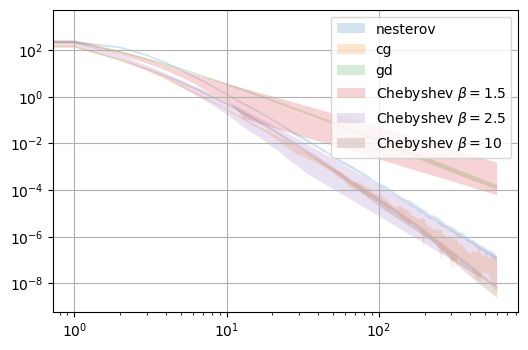
\includegraphics[width= 5 cm]{imgs/mp/log grad.png}
    
    
    \caption{Rates for a synthetic problem, simulating the Marchenko Pastur distribution. \textit{Left:} function value. \textit{Right}: gradient norm}
    \label{fig:my_label}
\end{figure}


\begin{figure}[H]
    \centering
    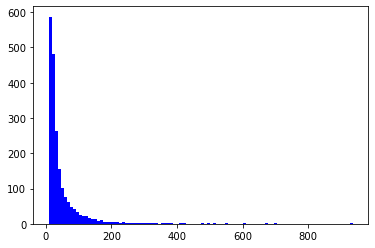
\includegraphics[width=5 cm]{imgs/inception/spectrum.png}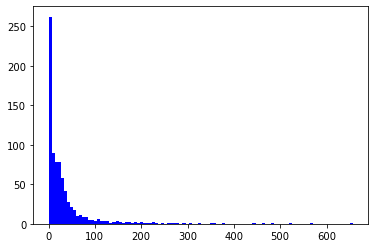
\includegraphics[width= 5 cm]{imgs/mnist/spectrum.png}
    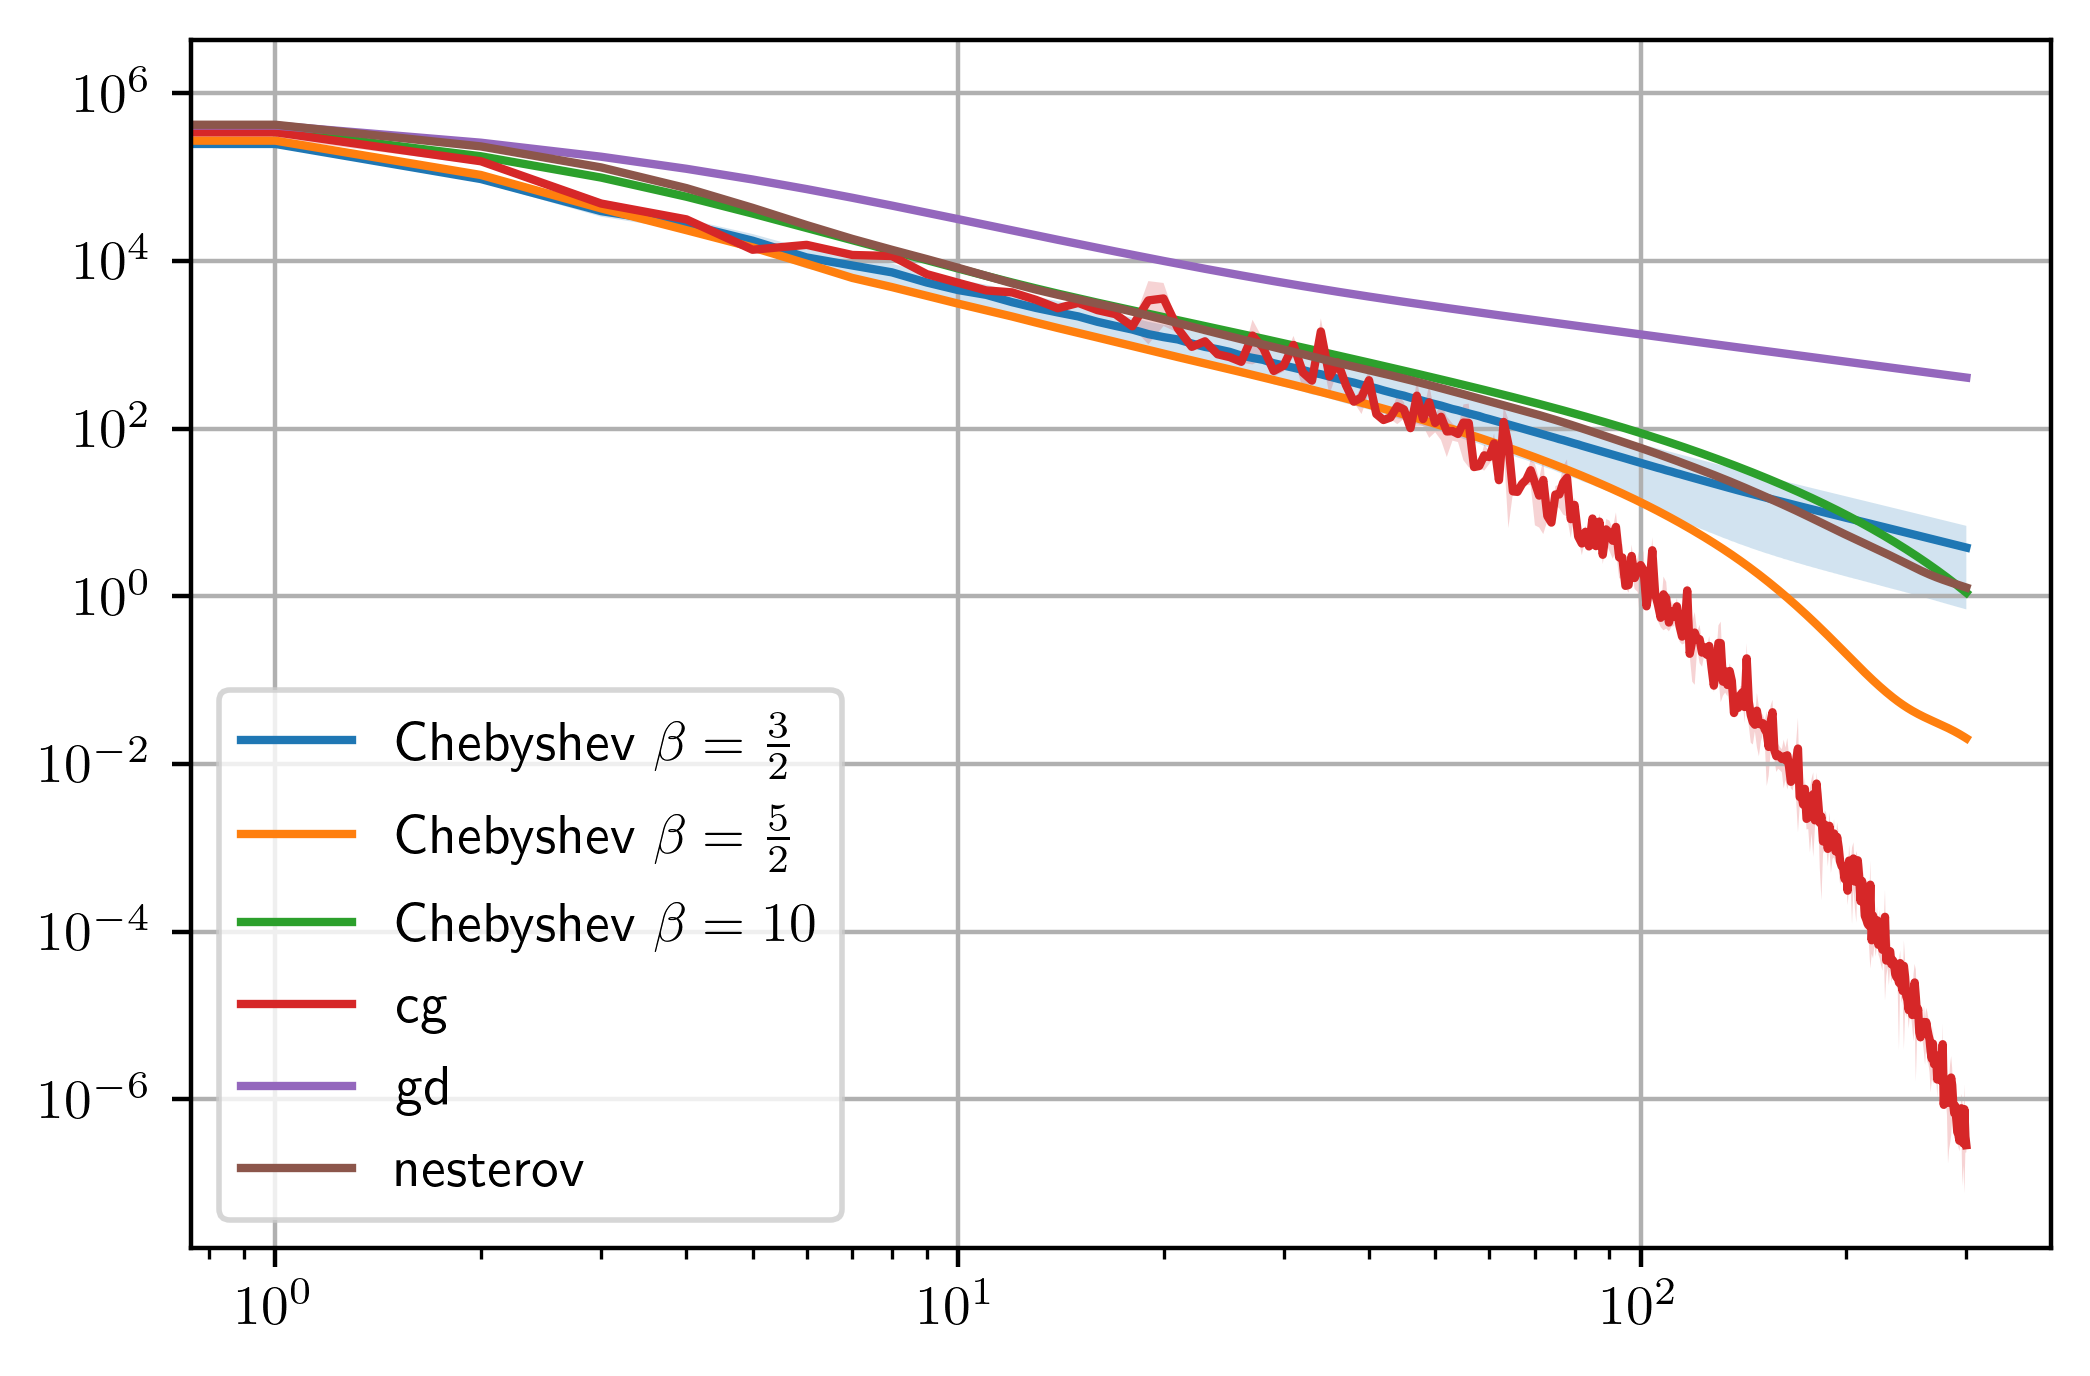
\includegraphics[width=5 cm]{imgs/inception/log grad.png}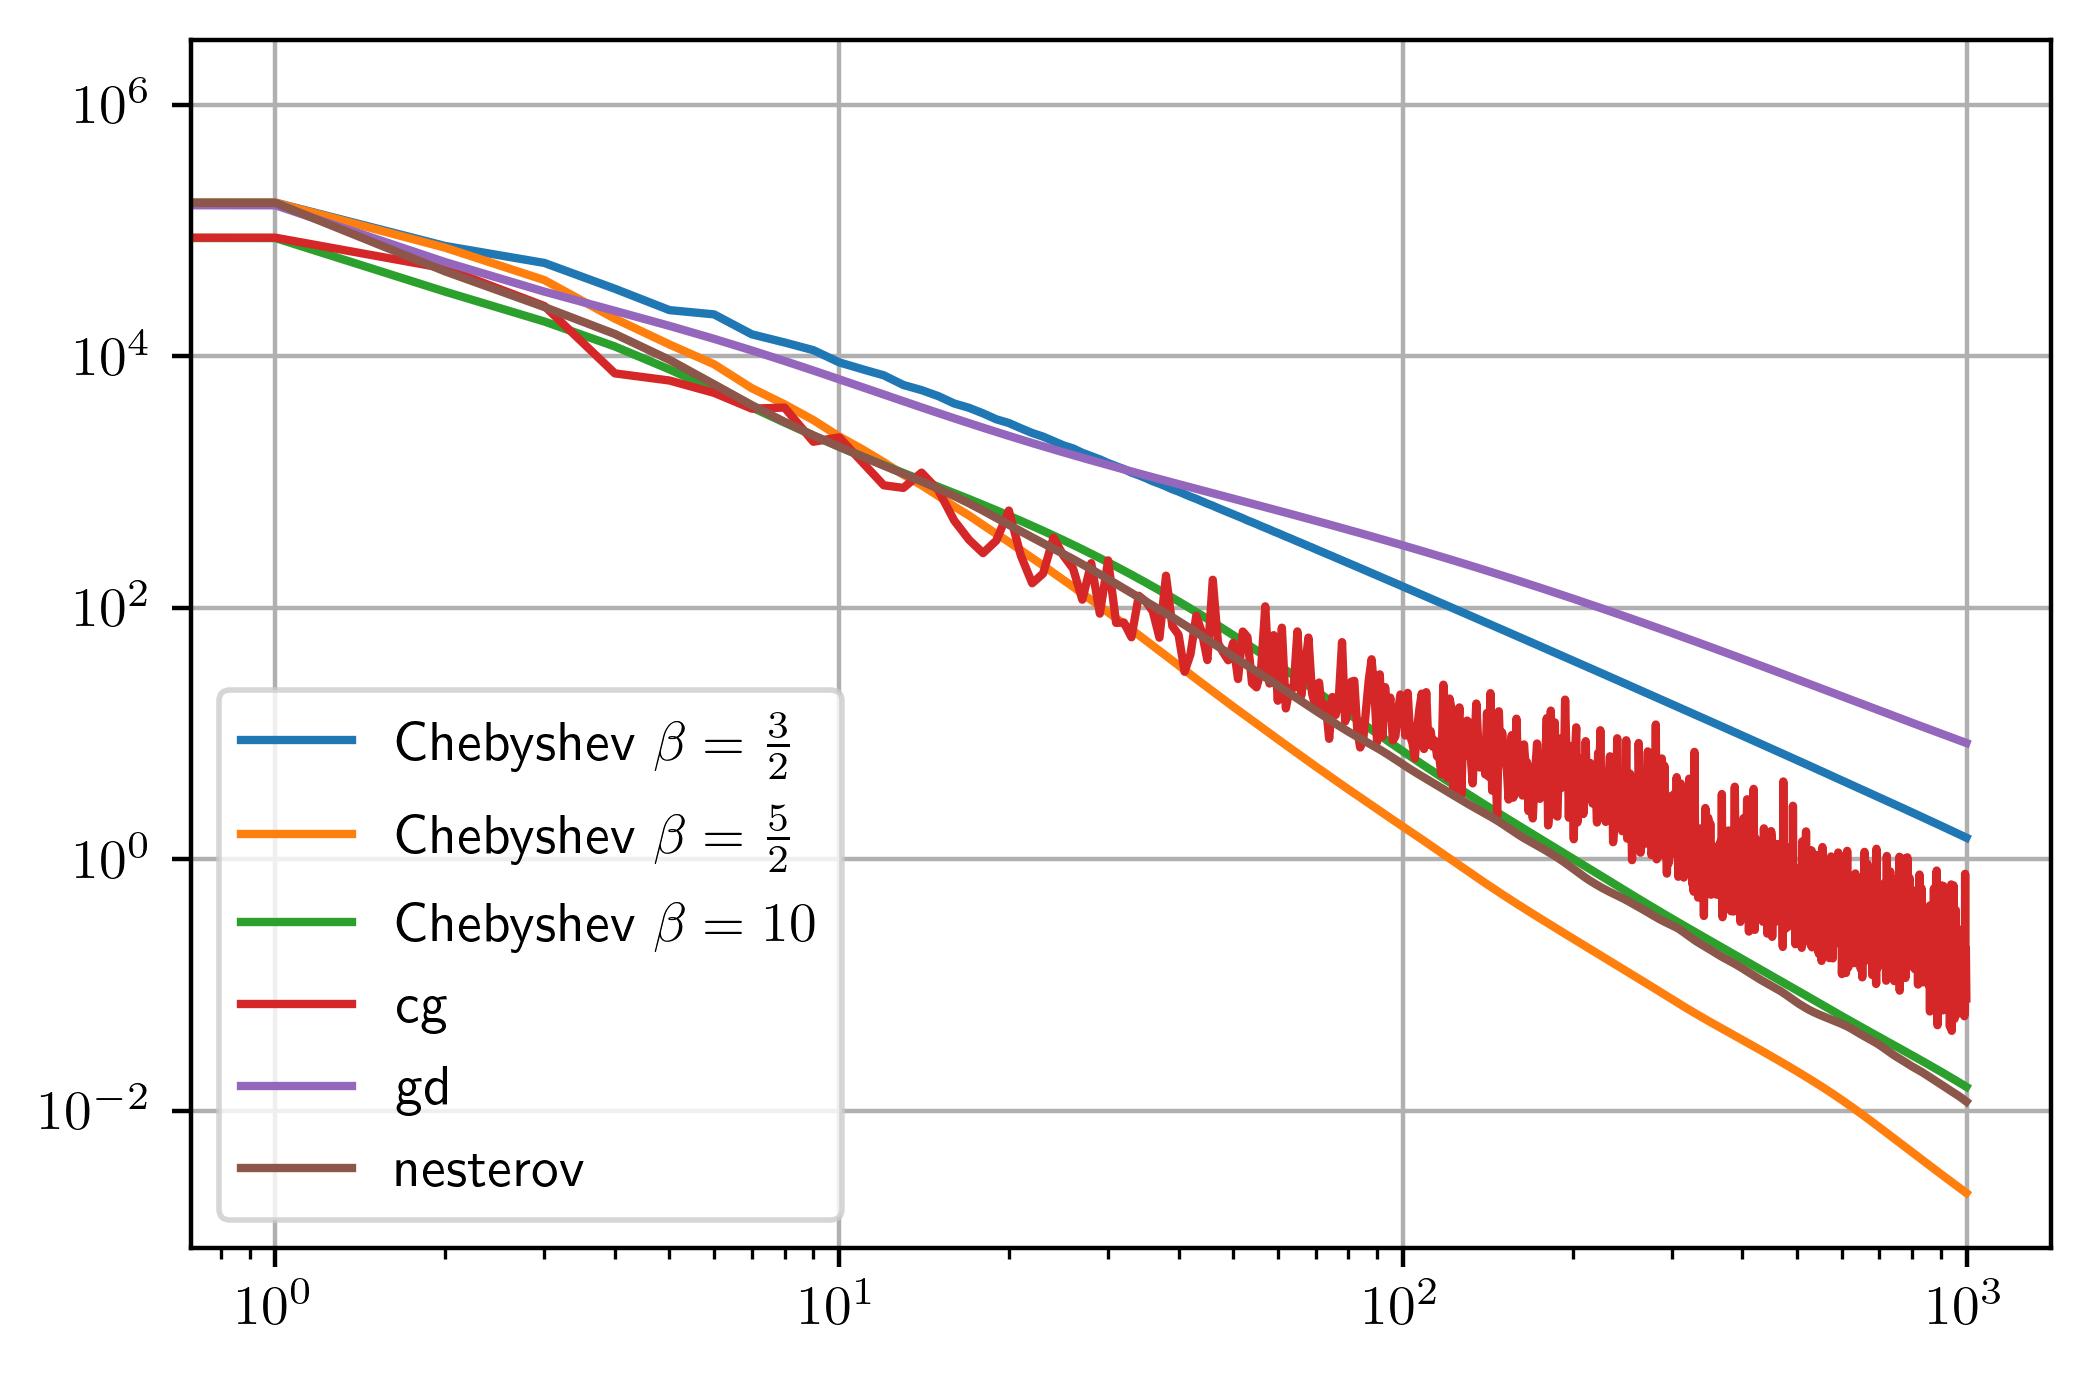
\includegraphics[width= 5 cm]{imgs/mnist/grad log.png}
    
    
    \caption{Spectrum and gradient norm rates for regression problems. \textit{Left:} CIFAR-10 Inception features \textit{Right}: MNIST features}
    \label{fig:my_label}
\end{figure}


\begin{figure}[H]
    \centering
    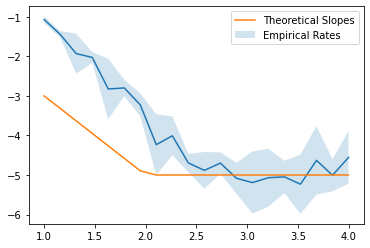
\includegraphics[width=5 cm]{imgs/theo vs practic.png}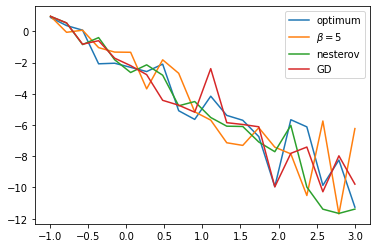
\includegraphics[width= 5 cm]{imgs/slopes.png}
    
    
    \caption{Rates for a synthetic problem, simulating the Marchenko Pastur distribution. \textit{Left:} function value. \textit{Right}: gradient norm}
    \label{fig:my_label}
\end{figure}

\begin{table}[H]
    \centering
    \begin{tabular}{c|c|c|c}
         $(\tau,\xi)$/Method& Chebyshev ($\frac{1}{2},\frac{5}{2}$) & Chebyshev ($\frac{1}{2},\frac{7}{2}$) &  Nesterov  \\
         \hline
         ($\frac{3}{2},\frac{1}{2}$)&$t^{-3.96}$? & $t^{-4.93}$ & $t^{-4.01}$\\
         \hline
         ($\frac{1}{2},\frac{1}{2}$)&$t^{-3.00}$ & $t^{-2.83}$ & $t^{-2.68}$
         
    \end{tabular}
    \caption{Caption}
    \label{tab:experimental rates}
\end{table}
%%Chebyshev \beta=5/2 is not giving the expected gradient performance ...


\section{Conclusion}
\printbibliography
\appendix
\newpage
\section{Proofs of Section 2}
\metrics*
\begin{proof}
\newcommand\xinit{\xx_0-\xx^\star}
We remark that by the definition of the expected spectral distribution $\mu$ of $\HH$, we have for continuous $g$:
\begin{equation}
    \EE_H[g(tr(\HH))]=\int g(\lambda)\dif mu(\lambda)
\end{equation}
We know that $\xx_t-\xx^\star=P_t(\HH)(\xinit)$. We can write $||\xx_t-\xx^\star||^2$ in terms of a trace and use the independence of $\HH$ and $\xinit$ to connect it to the e.s.d.:
\begin{align}
    \mathbb{E}||\xx_t-\xx^\star||^2&=\EE[ tr((\xinit)^TP_t(\HH)^2(\xinit))] \\
    &=\EE_{\HH,\xinit} [tr(P_t(\HH)^2(\xinit)(\xinit)^T]\\
    &=\EE_\HH\left[P_T(\HH)^2\EE_{\xinit}[(\xinit)(\xinit)^T])\right]  \\
    &=R^2\EE_\HH[P_t(tr(\HH))^2]=R^2 \int P_t(\lambda)^2\dif\mu(\lambda)
\end{align}
For the gradient and function value the reasoning is the same by noticing:
\begin{align}
    \EE[f(\xx_t)-f(\xx^\star)]&=\EE[ tr((\xinit)^TP_T(\HH)\HH P_t(\HH)(\xinit))]\\
    &=\EE_\HH[(\lambda P_t)(\tr(H))^2] 
\end{align}
Where $\lambda P_t$ is the polynomial defined by the multiplication. As $\nabla f(\xx_t)=\HH(\xx_t-\xx^\star)$
\begin{align}
    \EE||\nabla f(\xx_t))||^2&=\EE[ tr((\xinit)^TP_T(\HH)\HH^2 P_t(\HH)(\xinit))]\\
    &=\EE_\HH[(\lambda^2 P_t)(\tr(H))^2]
\end{align}


\end{proof}

\optimality*
\begin{proof}
We differentiate the expression for the metrics w.r.t. to the coefficients of the polynomials:
\begin{align*}
    \frac{d}{da_k}\left(\int \lambda^lP_t^2(\lambda)d\mu(\lambda)\right)&=\int\lambda^l\frac{\dif}{\dif a_k}\left(\sum_{k=0}^t a_k\lambda^kP_t(\lambda) \right) \dif \mu(\lambda)=
    \\&=2\cdot\left(\int \lambda^{l+k}P_t(\lambda)d\mu(\lambda)\right)=0
\end{align*}
This means that $P_t(\lambda)$ is orthogonal to any polynomial of degree $t-1$  w.r.t to the intern product $\langle.,.\rangle_{\lambda^{l+1}d\mu}$

\end{proof}

\section{Coefficients  of the Jacobi Method}
We'll first state two lemmas that allow us to construct the optimal polynomials. With them in hand the procedure is trivial.

\begin{lemma}
Let $(\tp_t)$ be a family polynomials  following  
\begin{equation*}
    \tp_t(\lambda)=(\alpha_t+\beta_t\lambda)\tp_{t-1})\lambda)+\gamma_t\tp_{t-2}(\lambda)
\end{equation*}
With $\tp_0$ a constant polynomial and $\tp_t\neq0, \forall t$. Then:
\begin{equation}
    P_t(\lambda)=(a_t+b_t\lambda)P_{t-1}(\lambda)+(1-a_t)P_{t-2}(\lambda)
\end{equation} Is the recurrence for $P_t(\lambda)=\tp_t(\lambda)/\tp_t(0)$. With:
\begin{align}
    a_t&=\delta_t\alpha_t \\
    b_t&=\delta_t\beta_t \\
    \delta_t&=(\alpha_t+\gamma_t\delta_{t-1}) \hspace{0.5 cm } (\delta_0=0)
\end{align}
\end{lemma}
The proof of this is presented in \cite{pedregosa2020acceleration}. Further, we know how to compute the recurrence for the polynomials of a shifted distribution:
\begin{lemma}

Let $(\tp_t)$ be a family polynomials orthogonal w.r.t  following  
\begin{equation}    \label{rec}
    \tp_t(\lambda)=(\alpha_t+\beta_t\lambda)\tp_{t-1}(\lambda)+\gamma_t\tp_{t-2}(\lambda
\end{equation}
And define polynomials $P_t$ s.t. :
$$
P_t(m(\lambda))=\tp_t(\lambda)
$$
With $m(\lambda)=a\lambda+b$ a non singular affine transform. Then $P_t$ follows a recurrence like in eq. \eqref{rec}, with:
\begin{align}
    \alpha_t'&=\alpha_t+b\beta_t \\
    \beta'_t&=a\beta_t\\
    \gamma'_t&=\gamma_t
\end{align}
\end{lemma}
The lemma is self-evident by considering eq. \eqref{rec} with argument $m^{-1}(\lambda)$
\paragraph{}
\label{jacobi recurrence}
Then to get  the recurrence relation for the residual polynomial w.r.t $x^\beta(L-x)^\alpha$, we begin by the standard jacobi polynomials, which are orthogonal w.r.t $(1-x)^\alpha(1+x)^\beta$ and follow a recurrence according to $\alpha_t,\beta_t,\gamma_t$ below, shift the distribution according to $\eta(x)\ldots$, and then transform to the residual ones:
\begin{prop}
The residual polynomials w.r.t. $d\mu(\lambda)=\lambda^\beta(L-\lambda)^\alpha$, follow the recurrence:
\begin{equation*}
    P_t(\lambda)=(a_t+b_t\lambda)P_{t-1}(\lambda)+(1-a_t)P_{t-2}(\lambda)
\end{equation*}
With:
\begin{align}
    \alpha_t&=\frac{(\alpha^2-\beta^2)(2n+\alpha+\beta+1)}{
            2(n+1)(n+\alpha+\beta+1)(2n+\alpha+\beta)} \\
        \beta_t&=\frac{(2n+\alpha+\beta+1)(2n+\alpha+\beta+2)}{
            (2(n+1)(n+\alpha+\beta+1)} \\
        \gamma_t&=-\frac{(n+\alpha)(n+\beta)(2n+\alpha+\beta+2)}{
            (n+1)(n+\alpha+\beta+1)(2n+\alpha+\beta)} \\
        \tilde{a}_t&=\alpha_t-\beta_t \\
        \tilde{b}_t&=\frac{2}{L}\beta_t \\
        \delta_t&=\frac{1}{\tilde{a}_t+c_t\delta_{t-1}}  \hspace{1 cm} (\delta_0=0)\\
        a_t,b_t&=\delta_t\tilde{a}_t,\delta_t\tilde{b}_t
\end{align}


\end{prop}

\section{Proofs of section 3}
In the following we'll consider shifted versions of the spectral distributions. This shift is written as an affine transform $m(\lambda):[0,L]\rightarrow [-1,1]$ because most results in the theory of orthogonal polynomials are stated in terms of distributions supported in $[-1,1]$. \\
This can be seen as an additional layer of abstraction because the quantities evaluated with the shifted distributions and polynomials are proportional, i.e. if $P_t(x)=\tp_t(m(x))$ and $\mu'(x)=\tmu'(m(x))$:
\begin{equation}
    \int P_t^2(x)\mu'(x)\dif x\propto \int \tp_t^2(x)\tmu'(x)\dif x
\end{equation}
So all the asymptotics are the same and we consider $\nu$ restricted to $[-1,1]$. 
The Jacobi polynomials $\JP$ are orthogonal w.r.t; $d\mu(x)=(1-x)^\alpha(1+x)^\beta$, we note that most results give them in terms of normalization $\tp_t^{\alpha,\beta}(-1)=(-1)^n\binom{t+\beta}{t}$. We'l write $\tp^{\alpha,\beta}_t$ for this normalization and $\JP_t$ for the residual polynomials
\robustjacobi*
\begin{proof}
We'll prove that for any $\alpha$ and $\beta$, $\xi,\tau>-1$, $l>0$ and $\nu$ following Assumption \ref{assumption}, we have:
\begin{equation*}
    \int P_t^{\alpha,\beta}(x)^2x^l d\nu_{\tau,\xi-l}(x) \sim  L^lC^{\alpha,\beta}_\nu\left\{
	\begin{array}{ll}
		  t^{-1-2\beta}& \mbox{if } 
		  \alpha<\tau+1/2 \text{ and } \beta <\xi+1/2\\
		  t^{-2(\xi+1)}\log t& \mbox{if } 
		  \alpha=\tau+1/2 \text{ and } \beta =\xi+1/2\\
		  t^{2(\max\{\alpha-\beta-\tau,-\xi\}-1)}& \mbox{if } 
		  \alpha>\tau+1/2 \text{ or } \beta >\xi+1/2
	\end{array}
\right.
\end{equation*}
We first state a lemma shown in \cite{van1995weak} relating to the weak convergence of the orthogonal polynomials:

\begin{lemma}
 Let $\mu$ be a measure and $(p_t)$ it`s family of orthonormal polynomials s.t.  $p_t$ follow the recurrence:
 \begin{equation*}
     xp_t(x)=a_tp_{t+1}(x)+b_tp_t(x)+a_{t-1}p_{t-1}(x)
 \end{equation*}
 and $a_t,b_t$ converge respectively to $a,b$. Then for any $f$  continuous and bounded:
\begin{equation}
    \int f(x)p_t^2(x)d\mu(x) \rightarrow \frac{1}{\pi}\int_{-1}^1 \frac{f(x)}{\sqrt{1-x^2}}dx   
\end{equation}
\label{wk}
\end{lemma} The normalization of $\tp^{\alpha,\beta} _t$ is s.t. \cite{szego1975orthogonal} (4.3.3):
\begin{equation}
    \int_{-1}^1\tp_t^{\alpha,\beta}(x)(1-x)^\alpha(1+x)^\beta \dif x=\frac{2^{\alpha+\beta+1}}{2n+\alpha+\beta+1}\frac{\Gamma(n+\alpha+1)\Gamma(n+\beta+1)}{\Gamma(n+1)\Gamma(n+\alpha+\beta+1)}=\Theta(t^{-1})
\end{equation}

The residual polynomials then are s.t. $|P^{\alpha,\beta}_t|=\Theta(t^{-\beta})\tp^{\alpha,\beta}_t$.\\
We also state the following result (Exercise 91, Generalisation of 7.34.1) from \cite{szego1975orthogonal}:
\begin{lemma}
We have:
\begin{align}
    \int_0^1(1-x)^\tauP_t^{\alpha,\beta}(x)^2dx &\sim\Theta( h_{\tau}^\alpha) \\
    h_{\tau}^\alpha&:=
\left\{
	\begin{array}{ll}
		t^{2(\alpha-\tau-1)}  & \mbox{if } \alpha>\tau+1/2 \\
		t^{-1}\log n   & \mbox{if } \alpha=\tau+1/2 \\
		t^{-1}   & \mbox{if } \alpha<\tau+1/2
	\end{array}
\right.
\end{align}
 \label{jacobi lemma}
\end{lemma}
Noting that $\tp^{\alpha,\beta}_t(x)=(-1)^t\tp_t^{\beta,\alpha}(-x)$, we can write:
\begin{equation}
    \int_{-1}^1\tp_t(x)^2(1-x)^\tau(1+x)^\xi dx = \Theta\left(\int_0^1(1-x)^\tau|\tp_t^{\alpha,\beta}(x)|^2dx\right) +\Theta\left(\int_0^1(1-x)^\xi|\tp_t^{\beta,\alpha}(x)|^2dx\right) \label{int decomp}
\end{equation}
We can then show our result for $\dif\nu_{\tau,\xi-l}(x)=x^{\xi-l}(L-x)^\alpha$ by carefully considering each of the cases on eq. \ref{jacobi lemma} and the maximum of each term in eq. \ref{int decomp}, and an added $t^{-2\beta}$ from the different normalization. \\
It rests to show that all cases can be brought down to this one. Indeed we show simply:
\begin{equation}
    \int_0^1 \tp_t^{\alpha,\beta}(x)^2\dif\nu_{\tau,\xi}(x)= \Theta\left(\int_0^1(1-x)^\tau\tp_t^{\alpha,\beta}(x)^2dx \right)
\end{equation}
And the rest follows from the same arguments. Let $\epsilon$ s.t.
\begin{equation}
    x\geq 1-\epsilon \Rightarrow |\dif\nu_{\tau,\xi}-A(1-x)^\tau|\leq  B(1-x)^\tau \label{eq: epsilon}
\end{equation}
We observe that for $0<x<1-\epsilon$, $f(x)=\frac{d\nu_{\tau,\xi}}{(1-x)^\alpha(1+x)^\beta}$ is bounded. \\
We get from an application of \ref{wk}, and the observation that $\tp_t^{\alpha,\beta}=\mathcal{N}_tp_t^{\alpha,\beta}$, with $\mathcal{N}_t=\Theta(t^{-1/2})$:
\begin{align}
    \underbrace{\int_0^1(1-x)^\tau\tp_t^{\alpha,\beta}(x)^2\dif x}_{\Theta( h_\tau^\alpha)}&=\underbrace{\int_0^{1-\epsilon}(1-x)^\tau\tp_t^{\alpha,\beta}(x)^2\dif x}_{\Theta( t^{-1})
    } +\int_{1-\epsilon}^1(1-x)^\tau\tp_t^{\alpha,\beta}(x)^2\dif x \Rightarrow\\
    &\int_{1-\epsilon}^1(1-x)^\tau\tp_t^{\alpha,\beta}(x)^2\dif x  =\Theta( h_\tau^\alpha) \\
    \int_0^1 \tp_t^{\alpha,\beta}(x)^2\dif\nu_{\tau,\xi}(x)&=
    \underbrace{\int_0^{1-\epsilon} \tp_t^{\alpha,\beta}(x)^2 f(x) (1-x)^\alpha(1+x)^\beta\dif x)}_{\Theta( t^{-1})
    }+\Theta\left(
    \underbrace{\int_{1-\epsilon}^1(1-x)^\tau\tp_t^{\alpha,\beta}(x)^2\dif x}_{\Theta( h_\tau^\alpha)}\right)
\end{align}


\end{proof}

\jacoptimal*
\begin{proof}
We'll prove that for $\tau,\xi>-1$ If $\alpha = \tau$ and $\beta = \xi+l+1$ (i.e., are optimal), the rate of convergence reads
\begin{equation}
    \min_{P_t(0)=1}\int P_t^2(\lambda)\lambda^ld\nu(\lambda)=\Theta\left( \int_{0}^l  \tp_t^{\alpha,\beta}(\lambda)^2(L-\lambda)^\tau\lambda^{\xi+l}\dif \lambda\right) =\Theta( t^{-2(\xi+l+1)})
\end{equation}
Showing the second equality is easy by considering theorem \ref{thm: jacobirat}, and that is further the minimum asymptotic rate for the Beta distribution. \\
As $\tp^{\alpha,\beta}_t$ has the same rate on $\nu$ as  on the Beta distribution , the minimum rate for $\nu$ is lower bounded by the r.h.s. \\
We argue that, setting $P^\nu_t=\frac{p^\nu}{}$ the optimal residual and orthonormal polynomials and $\mu_{\tau,\xi}$ the Beta distribution  w.r.t, $P^\nu_t$ must have the same rate on $\nu$ as it does on $\nu$. Indeed, setting $\epsilon_1,\epsilon_2$ as in eq. \ref{eq: epsilon}, we argue:
\begin{align}
    \int_{1-\epsilon_2}^{1}P_t^\nu(x)^2d\nu(x)&=\left(\Theta\int_{1-\epsilon_2}^{1}P_t^\nu(x)^2d\mu(x)\right)\\
    \int_{-1}^{-1+\epsilon_1}P_t^\nu(x)^2d\nu(x)&=\Theta\left(\int_{-1}^{-1+\epsilon_1}P_t^\nu(x)^2d\mu(x)\right)\\
    \int_{-1+\epsilon_1}^{1-\epsilon_2}P_t^\nu(x)^2d\nu(x)&=\Theta\left(\int_{-1+\epsilon_1}^{1-\epsilon_2}P_t^\nu(x)^2d\mu(x)\right)=\Theta\left(\frac{1}{p_t^\nu(-1)^2}\right)\\
\end{align}
Where the first two equations come from the fact that $\nu=\Theta(\mu)$ near $-1$ and $1$ and the third from lemma \ref{wk}.\\
This effectively upper bounds the rates on $\nu$ because the rates of $P_t^\nu$ on $\mu_{\tau,\xi}$ can't be lower than $-2(\xi+1)$.
\end{proof}




\worstcase *
\begin{proof}
rates]
We'll prove that:  $\sup_{x\in[0,L]}x^lP_t^{\alpha,\beta}(x)^2=O(L^lt^{v(\alpha,\beta,l)})$. Where:
\begin{equation}
    v(\alpha,\beta,l)=\left\{
    \begin{array}{cc}
           2(\alpha-\beta) &\text{if} \hspace{0.5 cm} \alpha>\beta-l \\
         -1-2\beta, \hspace{1 cm} &\text{if} \hspace{0.5 cm} \alpha\leq \beta-l\hspace{0.5 cm} \beta\leq l-\frac{1}{2}\\
         -2l, \hspace{1 cm} &\text{if} \hspace{0.5 cm} \alpha\leq\beta-l\hspace{0.5 cm} \beta\geq l-\frac{1}{2} 
    \end{array}
    \right . 
\end{equation}
From \cite{szego1975orthogonal}, Theorem 7.32.2, if $\theta<\frac{\pi}{2}$:
\begin{equation}
    \tp_t^{\alpha,\beta}(\cos \theta)=\left\{ 
    \begin{array}{cc}
         O(t^{-1/2})  \hspace{1 cm} &\text{if} \hspace{0.5 cm} \alpha < -\frac{1}{2} \\
         O(t^{\alpha})  \hspace{1 cm} &\text{if} \hspace{0.5 cm} \alpha \geq -\frac{1}{2} , 0\leq\theta\leq ct^{-1} \\
         \theta^{-
         \alpha-1/2}O(t^{-1/2})  \hspace{1 cm} &\text{if} \hspace{0.5 cm} \alpha \geq -\frac{1}{2} , \theta> ct^{-1}
    \end{array}
    \right .
\label{lemma: worst case}
\end{equation}
We observe that, from the symmetry of the jacobi polynomials:
\begin{equation}
    \sup_{x\in[0,L]}x^lP_t^{\alpha,\beta}(x)^2 =\Theta\left( \max\left\{\sup_{x\in[0,1]}P_t^{\alpha,\beta}(x)^2,\sup_{x\in[0,1]}(1-x)^lP_t^{\beta,\alpha}(x)^2\right\}\right)
\end{equation}
The $(1-x)^l$ term,  corresponds to $(2\sin(\frac{\theta}{2}))^l$ in the variable $\theta$, which is $O(\theta^{2l})$. The rest follows from carefully considering the expressions given by eq. \ref{lemma: worst case}.
\end{proof}


\nesterovrates * 


\begin{proof}
We'll prove:
\begin{equation}
    \int_0^1P_t^{\text{Nes}}(\lambda)^2\lambda^l\dif\nu_{\tau,\xi-l}\sim C'_\nu
    \Big\{\begin{array}{ll}
          t^{-2(\xi+1)}& \mbox{if } 
		  0<\xi<1/2  
		  t^{-3}\log t& \mbox{if } 
		  \xi=1/2\\
		  t^{-(\xi+5/2)}& \mbox{if } 
		  \xi>1/2
	\end{array}
\end{equation}
\cite{paquette2020halting} has shown that the nesterov polynomials $P_t$ are asymptotically, in $t$:
\begin{equation}
    P_t(\lambda)\sim\frac{2J_1(t\sqrt{\alpha\lambda})}{t\sqrt{\alpha\lambda}}e^{-\alpha\lambda t/2}
\end{equation}
In the sense that:
\begin{equation}
    \int_0^1u^{l}[\Tilde{P_t^2(u)}-\frac{4J_1^2(t\sqrt{u})}{t^2u}e^{-u t}\dif\mu_{MP}(u)=O(t^{-(l+25/12))}
\end{equation}
The arguments can be easily used to show that such an integral is $O(t^{ -(\alpha+l+31/12)})$ when evaluated wrt a general $\dif\mu$ s.t $\mu'=\Theta(\lambda^\alpha)$ near $0$. \\
We can thus consider our integral  of interest substituting $P_t^\text{Nes}$ by it's Bessel asymptotic and dividing it into three regions, corresponding to two different regimes for the Bessel function. One of the regions will give us the asymptotic and the others we'll bound.\\
We consider first, for some $\epsilon>0$:
\begin{equation}
    \int_{\frac{\epsilon}{t}}^{\frac{\epsilon}{\sqrt{t}}} u^{\xi}\frac{4J_1^2(t\sqrt{u})}{t^2u}e^{-u t}\dif u
\end{equation}
We note the asymptotic for $J_1^2$:
\begin{equation}
    J_1^2(\sqrt{tv}) \sim \frac{1}{\pi\sqrt{tv}}(1+\cos(2\sqrt{tv}+2\gamma))
\end{equation}
Doing the change of variable $v=tu$, and identifying the upper limit of the interval, which is $\epsilon t^{1/2}$ to $\infty$:

\begin{align}
    \int_{\frac{\epsilon}{t}}^{\frac{\epsilon}{\sqrt{t}}} u^{\xi}\frac{4J_1^2(t\sqrt{u})}{t^2u}e^{-u t}\dif u &=\Theta\left(
    t^{-2-\xi}\int_\epsilon^\infty v^{\xi-1}J_1^2(\sqrt{tv})e^{-v}\dif v\right)\\
    &=\Theta\left( t^{-2-\xi}\int_\epsilon^\infty v^{\xi-1}\frac{1}{\pi\sqrt{tv}}e^{-v}\dif v \right)\\
    &=\Theta\left(t^{-\frac{5}{2}-\xi}\underbrace{\int_\epsilon^\infty v^{\xi-\frac{3}{2}}\frac{1}{\pi\sqrt{tv}}e^{-v}\dif v}_{\Gamma(\xi-\frac{1}{2},\epsilon) }\right)
\end{align}
Where the cosinus term goes to $0$ from the Riemann-Lebesgue lemma and $\Gamma$ is the incomplete Gamma function.\\
The term corresponding to the interval $[\epsilon t^{-1/2},1]$ is exponentially small. Indeed, because of the exponential $e^{-ut}$ it is  $O(e^{-\epsilon\sqrt{t}})$. This shows that the integral concentrates in a region that is closer and closer to $0$ and that only the behaviour of the distribution near $0$ matters.\\
We have for the $[0,\frac{\epsilon}{t}]$ region, doing the change of variables $v=t^2u$:
\begin{equation}
    \int_0^{\frac{\epsilon}{t}} u^{\xi}\frac{4J_1^2(t\sqrt{u})}{t^2u}e^{-u t}\dif u &=\Theta\left(
    t^{-2(\xi+1)}\int_0^{t\epsilon} v^{\xi}\frac{J_1^2(\sqrt{v})}{v}e^{-\frac{v}{t}}\dif v\right)
\end{equation}
And the $e^{\frac{-v}{t}}$ is $\Theta(1)$. We have the following Bessel asymptotics:
\begin{align}
    \frac{J_1^2(\sqrt{v})}{v}&\sim \frac{1}{4}, \hspace{2 cm} v\rightarrow 0 \\
    \frac{J_1^2(\sqrt{v})}{v}&= O(v^{-3/2}), \hspace{1.0 cm} v\rightarrow \infty
\end{align}
So we divide this integral aswell:

\begin{align}
    t^{-2(\xi+1)}\int_1^{t\epsilon} v^{\xi}\frac{J_1^2(\sqrt{v})}{v}e^{-\frac{v}{t}}\dif v
    &=\Theta\left(t^{-2(\xi+1)}\int_\epsilon^{t\epsilon} v^{\xi-\frac{3}{2}}\dif v\right) =\Theta\left( I_\xi(t)t^{-\xi-\frac{5}{2}}\right)\\
    t^{-2(\xi+1)}\int_0^{1} v^{\xi}\frac{J_1^2(\sqrt{v})}{v}e^{-\frac{v}{t}}\dif v
    &=\Theta\left(t^{-2(\xi+1)}\int_0\epsilon^{1} v^{\xi} \dif v\right) =\Theta\left( t^{-2(\xi+1)}\right)
\end{align}
Where $I_\xi(t)=\log t$ if $\xi=\frac{1}{2}$ and $1$ otherwise. \\
The nesterov rate is then $I_\xi(t)t^{-\xi-\frac{5}{2}}$ if $\xi\geq\frac{1}{2}$ and $t^{-2(\xi+1)}$ if $0<\xi<\frac{1}{2}$
\end{proof}


%%What happens when L is not properly set?
%% nesterov rates with tau< 1/2
\end{document}